\documentclass[11pt,a4paper]{article}
\usepackage{enumitem,amssymb,graphicx,epstopdf,authblk,minted,expl3,listings,hyperref}
\usepackage[T1]{fontenc}
\usepackage[utf8]{inputenc}
\usepackage[lmargin=2.5cm, rmargin=2.5cm,tmargin=3cm,bmargin=2.5cm]{geometry}
% You must have pygments installed for this program to work
% Assuming a working python installation, rin $ pip install pygments
% Make sure pygmentize is available in your latex compiler/text editors $PATHs

\begin{document}

\title{Introduction to Micro-controllers}
\date{\today} 
\author{Andres LaRosa}
\author{Bret Comnes}
\affil{Portland State University}
\maketitle

\section{Introduction} % (fold)
\label{sec:introduction}

Microcontrollers are small computers designed to go where desktop computers dare not go.  They come in all shapes, sizes, and layouts.  Usually, they are quite small and use less power than traditional computers.  Microcontrollers are often deployed in an `appliances' and serve an unmodifiable dedicated purpose, such as keeping track of what spin cycle your washing machine is on, or how much time is left before it should turn off your microwave oven.  Make no mistake however, these are general purpose computers.  The other major difference between a microcontroller and traditional computers is that they they come with an array of analog and digital input and outputs. These inputs and outputs can be used to read environmental data from sensors, talk to other computers or devices and electronically control other systems which provide environmental outputs such as a LCD screen, mechanical switches or servo motors etc.  \cite{wpmicro}

Getting started with microcontrollers can be tedious process, as they can require a number of supporting circuits, USB controllers, programmers, boot-loaders and power supplies just to load your first program onto the microcontroller chip.  Often times you will start with a prototyping board, which puts all of the necessary components in a convenient ready to use package.

\subsection{Arduino} % (fold)
\label{sub:arduino}

\begin{figure}[htbp]
	\centering
		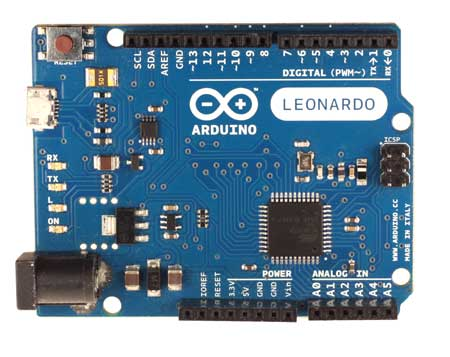
\includegraphics[height=2.7in]{figures/ArduinoLeonardoFront_2_450px.jpg}
	\caption{Arduino Leonardo\cite{leonardo}}
	\label{fig:figures_ArduinoLeonardoFront_2_450px}
\end{figure}


\begin{quote}
\emph{``Arduino is a tool for making computers that can sense and control more of the physical world than your desktop computer. It's an open-source physical computing platform based on a simple microcontroller board, and a development environment for writing software for the board.''} -- Arduino.cc\cite{arduino_guide}
\end{quote}

This lab will be using the Arduino Leonardo Microcontroller\cite{leonardo}.  It is similar to the Arduino Uno\cite{uno}, with the major difference being that it uses SMT\cite{smt} instead of the older ``thru-hole''\cite{th} technology in order to reduce cost.

Arduino drastically lowers the difficulty of getting started with a microcontroller (compared to to plain ATMEGA/PIC/ARM chips), as it provides all the necessary tools to start making the microcontroller do interesting things without nearly all the setup of just a plain microcontroller chip.

Arduino is based around an 8-bit Atmel AVR microcontroller, and has supporting systems like a boot loader for uploading programs, a USB controller as well as a barrel jack for external power.

It is programmed using a language that is based off of C++ and uses a fork of the Processing IDE used for writing, compiling and uploading your programs to the board.  Many Arduino projects you will find will rely on programs running on your computer using Processing, but can interface with any serial enabled programs.\cite{processing}

% subsection arduino (end)

% section introduction (end)


\section{Getting Started} % (fold)
\label{sec:getting_started}

\subsection{Setting up your software} % (fold)

This lab is based off of the Arduino 1.0.3 software which can be downloaded for free from the Arduino website.\cite{arduino_dl}  Unlike other embedded systems development environments, the Arduino software is quick to download and set up, and has zero cost associated with the software which makes it a convenient to work with when your primary goal is to come up with a working prototype quickly and cheaply.

It also has a large community and a massive pool of example programs and libraries.

\subsection{Find a Computer} % (fold)
\label{sub:find_a_computer}
You are free to use your own laptop or one of the classroom computers.  Plug your Arduino into the computer using the micro USB cable.  \textbf{Please be careful with the delicate connectors.}

% subsection find_a_computer (end)

\subsection{Download and Launch the Arduino Software} % (fold)
\label{sub:download_and_launch_the_arduino_software}
Visit \url{http://arduino.cc/en/Main/Software} and downloaded the latest Arduino software\cite{arduino_dl}.  If you have decided to use your own Arduino, make sure you find the necessary USB drivers if you have a board that is older than the Uno.

% subsection download_and_launch_the_arduino_software (end)

\subsection{Selecting the Board} % (fold)
\label{sub:selecting_the_board}
Once the IDE is open, navigate to the toolbar and select the board you are working with from \textbf{Toolbar $\rightarrow$ Tools $\rightarrow$ Board $\rightarrow$ Arduino Leonardo}.  If you are using a different board , select the one you have from this list instead.  This step may vary from system to system as well, but pick the option most similar to this write up.

% subsection selecting_the_board (end)

\subsection{Selecting a Serial Port} % (fold)

\label{sub:selecting_a_serial_port}
This step varies from system to system.  In this step, we tell the computer which serial port that the Arduino chip can be reached at, for programing the board, as well as talking to it during runtime.
    \begin{figure}[htbp]
        \centering
            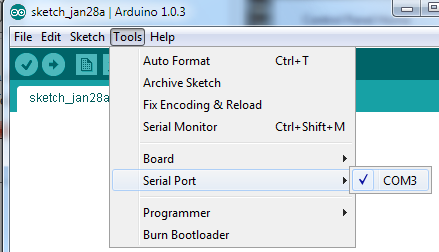
\includegraphics[height=2in]{figures/port-windows.png}
            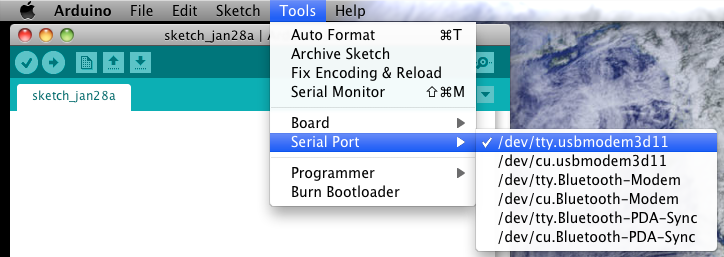
\includegraphics[height=1.5in]{figures/port-osx.png}
        \caption{Port Selection in Windows and OS X}
        \label{fig:figures_port}
    \end{figure}

\subsubsection{Windows} % (fold)

\label{ssub:windows}
Select \textbf{Toolbar $\rightarrow$ Tools $\rightarrow$ Serial Port $\rightarrow$ COM3} where COM3 is the serial port that has been assigned to your Arduino by windows.  You should only have one port available.

% subsubsection windows (end)

\subsubsection{OS X} % (fold)
\label{ssub:os_x}
Select \textbf{Toolbar $\rightarrow$ Tools $\rightarrow$ Serial Port $\rightarrow$ /dev/tty.usbmodem3d11} where COM3 is the serial port that has been assigned to your Arduino by windows.  You should only have one port available.

% subsubsection os_x (end)

% subsection selecting_a_serial_port (end)

\subsection{Uploading your first program} % (fold)
\label{sub:uploading_your_first_program}
Next we will open an example program, verify that it compiles, then upload it to our board.


Navigate to \textbf{Toolbar $\rightarrow$ File $\rightarrow$ Examples $\rightarrow$ 01. Basics $\rightarrow$ Blink}.  Press the verify button.  It should compile the sketch and return a `Done compiling' message.  If you get an error, something went wrong.

    \begin{figure}[htbp]
        \centering
            
\includegraphics{figures/verify.png}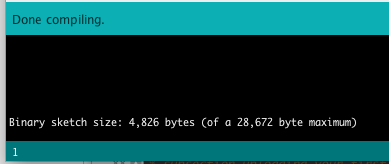
\includegraphics{figures/compile.png}
        \caption{Verify Button (Left) Compile Success Message (Right)}
        \label{fig:figures_verify}
    \end{figure}

If that completed, go ahead and upload the program to the board by pressing the upload button (the button right next to verify button) and it should provide a similar completion message after a few moments.  The LEDs on the Arduino will blink during the upload, but should settle down after a few seconds.  See Figure~\ref{fig:figures_verify}.  
    
Once the program you uploaded is running, the LED labeled `L' on your Arduino should be slowly blinking.  This LED labeled `L' is wired to Pin 13 on the Arduino, a digital pin with a resistor built in that so that LEDs can be added easily.  \textbf{Go ahead and add an LED between Pin 13 and GND}.  It should blink at the same rate as the `L' LED on the board.

% subsection uploading_your_first_program (end)


Congratulations!  You now have a working Arduino that is talking to the Arduino IDE.

% subsection setting_up_your_software (end)

% section getting_started (end)

\section{Programming Arduino} % (fold)
\label{sec:programming_arduino}

Arduino is based off the Processing\cite{processing} programming language, and has some similarities to C, however much of the language has been simplified from C.  In this section we will go over the basics of the language, look at some simple examples of code and even write some of our own.

\subsection{The Bare Minimum} % (fold)
\label{sub:the_bare_minimum}

The bare minimum code you need for an Arduino program is presented in Figure~\ref{fig:bare}.

\begin{figure}[htbp]
	\centering
\begin{minted}[mathescape,
				linenos,
				numbersep=5pt,
				gobble=0,
				frame=lines,
				framesep=2mm]{c}
void setup() {
// put your setup code here, to run once:
}
void loop() {
// put your main code here, to run repeatedly: 
}
\end{minted}
	\caption{The minimum Amount of code for an Arduino Program}
	\label{fig:bare}
\end{figure}

There are two parts to this minimum program, the \texttt{void setup() \{\}} section and the \texttt{void loop() \{\}} section.  When your program runs, It starts executing your code, line by line, starting in the \texttt{void setup()} section, inside the brackets, \texttt{\{\}}, that follow.  Your program will execute any code that is in this section, and when it gets to the end, will begin executing the code inside \texttt{void loop() \{\}}, until it gets to the end of the available instructions, at which point, the program starts back over in at the beginning of \texttt{void loop() \{\}}, retaining any variables or settings from prior lines of code.

Lets look at a simple example, that you should already have pulled up, the \texttt{Blink} program, which is found in Figure~\ref{fig:blink}.  If you still need to open this, refer to Section~\ref{sub:uploading_your_first_program}.

% subsection the_bare_minimum (end)


\section{Understanding the Blink Program} % (fold)
\label{sec:understanding_the_blink_program}

\begin{figure}[htbp]
	\centering
\begin{minted}[mathescape,
				linenos,
				numbersep=5pt,
				gobble=0,
				frame=lines,
				framesep=2mm]{c}
/*
  Blink
  Turns on an LED on for one second, then off for one second, repeatedly.
 
  This example code is in the public domain.
 */
 
// Pin 13 has an LED connected on most Arduino boards.
// give it a name:
int led = 13;

// the setup routine runs once when you press reset:
void setup() {                
  // initialize the digital pin as an output.
  pinMode(led, OUTPUT);     
}

// the loop routine runs over and over again forever:
void loop() {
  digitalWrite(led, HIGH);   // turn the LED on (HIGH is the voltage level)
  delay(1000);               // wait for a second
  digitalWrite(led, LOW);    // turn the LED off by making the voltage LOW
  delay(1000);               // wait for a second
}
\end{minted}
	\caption{The Blink Program in all its glory}
	\label{fig:blink}
\end{figure}

If a block of text is wrapped in \texttt{/* */}, such as lines 1 thru 6 in Figure~\ref{fig:blink} or has a \texttt{//} in front of it on one line, such as line 12, means it's a comment.  Comments are little notes you leave in your code.   They are not executed or interpreted by your program in any way.  It is good practice to add comments to your code.  They can help you think about your program, and will also remind you, and others that see your code, what the program does or how it works.

Running down lines 1-9, we see that this is all comments describing the function of the program, how it works, as well as the license.   The first piece of code we see is on line 10.


\subsection{Variables} % (fold)
\label{sub:variables}

\mint{c}|int led = 13;|

The first thing to notice, is that this code is not inside \texttt{void setup()} or \texttt{void loop()}.  That is because it is a variable and variables can be declared in the beginning of our program outside either loop. 

Variables are incredibly useful tools.  Variables store information that can be used later in the program as many times as you need.  They can be updated during run-time and cab be used to store values temporarily for repeated use.

Any variable we decide to use, we have to describe to our program.  This is referred to as declaring your variable.  \textbf{Variables are declared before your \texttt{void setup()} or \texttt{void loop()} sections.}  

Line 10 declares a variable named \texttt{led}, gives it a variable type of \texttt{int}, for integer, and then assigns it a value of 13.  This variable is used to reference the physical pin we will be using in our program.  It is used as an abstraction layer, so that if we ever go back and change which pin we want to use, we can update all the places in our program that reference this pin number simply by updating the initial variable value.

The basic syntax of a variable declaration is: 

\mint{c}|type variable_name = value;|

The available variable types can be found on the Arduino website \cite{ard_ref}

% subsection variables (end) 

\subsection{Pin Modes} % (fold)
\label{sub:pin_modes}

The next piece of code we arrive at is our \texttt{void setup()}.  Stepping inside the curly braces of this structure, we come to the following line:

\mint{c}|pinMode(led, OUTPUT);|

Digital pins can either read or write digital signals (0 or 5\emph{v}).  Before you do either, you must tell your program what you will be using the digital pin for.  This tells our program that the pin associated with the \texttt{led} variable will be a Digital output.

\mint{c}|pinMode([PIN-NUMBER], [PIN-TYPE]);|

Available pin modes can be found a the Arduino website.\cite{pin_mode}

Each pin has a name assigned to it.  Each pin on the Arduino has its name printed next to it, which can be seen in Figure~\ref{fig:figures_ArduinoLeonardoFront_2_450px}.  There are two primary types of pins:  Digital and Analog.  Digital pins simply have a number for a name, and analog pins have the letter A followed by a number for a name.

Digital pins can read or write digital signals varying from 0 to 5\emph{v}.  Some can also output PWM signals, a way to emulate analog voltage signals with a digital pin PWM capable digital pins have a \texttt{\~} printed next to their name on the board.  See Section~\ref{sub:understanding_pwm} for more information.

Analog Pins can read in analog voltages between 0v and 5v and converts them to a value that your program can use between 0 and 1023.  They do not need a pin mode set before reading within your program.

% subsection pin_modes (end)

\subsection{Generating Output} % (fold)
\label{sub:generating_output}

Once the pin mode is set, we exit our \texttt{void setup()} and enter our \texttt{void loop()}, the part of the program that will run over and over in an infinite loop. 

The first thing we do is execute: 

\mint{c}|digitalWrite(led, HIGH);|

\texttt{digitalWrite([PIN], [VALUE])} lets us set the output value of a digital pin that has been set to an OUTPUT type.  In this case, we write a value of \texttt{HIGH}, or 5\emph{v}, to the pin referred to by the \texttt{led} variable.  A value of \texttt{HIGH} would refer to 0\emph{v}.

The next part of the program tells the Arduino to wait for a period, before executing the next line of code.  \textbf{This period is equal to 1000ms, or 1 second.}

\mint{c}|delay(1000);|

After waiting for a second, we then write a value of \texttt{LOW} to our \texttt{led} pin, and then wait 1 more second.

\mint{c}|digitalWrite(led, LOW);|
\mint{c}|delay(1000);|

At this point, there is no more code left in our program, so it starts executing \texttt{void loop()} again.

% subsection generating_output (end)

Congratulations, you now should have some basic understanding of how an Arduino program is written.

% section understanding_the_blink_program (end)

\section{Modifying the Blink Program} % (fold)
\label{sub:modifying_the_blink_program}

Now you will try your hand at modifying the blink program.  What we are going to do is define a new variable called \texttt{wait}, give it a value, and then replace the delay time on the Arduino with our new variable. 

\subsubsection{Create a new variable} % (fold)
\label{ssub:create_a_new_variable}

Right below the \texttt{led} variable declaration, add a new variable named \texttt{wait} of type \texttt{int} and give it a reasonable value different than 1000 (like 100).  Also, add a comment describing what this variable is used for.
% subsubsection create_a_new_variable (end)

\subsubsection{Use your new variable} % (fold)
\label{ssub:use_your_new_variable}

We want to use this new variable to declare the time we wait in between turning our LED on and off.  Go ahead and replace the old delay values with your new variable name.  

% subsubsection use_your_new_variable (end)

\subsubsection{Verify and Upload your modified program} % (fold)
\label{ssub:verify_and_upload_your_modified_program}

The Arduino should still be set up from when you first uploaded the first blink program.  Verify your new program to see if it compiles.  If you get an error, check your work for syntax error.  Did you forget a semicolon or a brace?

Once your program verifies, and you are able to upload it to your board, you should start to see your LED blink faster or slower, depending on the value you defined your variable.

% subsubsection verify_and_upload_your_modified_program (end)

\subsubsection{Final modification} % (fold)
\label{ssub:final_modification}

Once you make your modification, you will have code that looks similar to Figure~\ref{fig:blinkmod}.
\begin{figure}[htbp]
	\centering
\begin{minted}[mathescape,
				linenos,
				numbersep=5pt,
				gobble=0,
				frame=lines,
				framesep=2mm]{c++}
int led = 13;
int wait = 100; // Time to wait before blinking

void setup() {                
  pinMode(led, OUTPUT);     
} 

void loop() {
  digitalWrite(led, HIGH);   
  delay(wait);  //Wait for the ammount declaired in the wait variable         
  digitalWrite(led, LOW);    
  delay(wait);  //Wait for the ammount declaired in the wait variable        
}
\end{minted}
	\caption{The modified Blink Program}
	\label{fig:blinkmod}
\end{figure}

% subsubsection final_modification (end)

% subsection modifying_the_blink_program (end)

% section programming_arduino (end)

\section{Using Inputs to Control Outputs} % (fold)
\label{sec:using_inputs_to_control_outputs}

\subsection{Understanding PWM} % (fold)
\label{sub:understanding_pwm}

Arduino cannot output true analog signals.  It can, however, generate Pulse Width Modulation (PWM) signals, which are similar to analog signals and can sometimes work interchangeably.  

\begin{quote}
\emph{``Pulse-width modulation uses a rectangular pulse wave whose pulse width is modulated resulting in the variation of the average value of the waveform'''} -- Wikipedia\cite{pwm}
\end{quote}

Basically, if driving an LED with a PWM signal, you are able to vary the brightness of the LED by having it blink really fast while varying the duration of each blink, resulting a brighter or dimmer output.  The result is that you can generate signals with similar properties as analog signals using pins only capable of switching between 0 and 5\emph{v}.

\subsubsection{Observing PWM} % (fold)
\label{sub:observing_pwm}

Load the \textbf{01.Basic $\rightarrow$ Fade} example program and upload it to your Arduino Board, and wire up the LED to the pin that is used in the program (this requires reading the program).  If it is a digital pin other than pin 13, you will need to add a $330\Omega$ resistor in series for good measure.  If you increase the delay time to \~80, you should be able to observe the PWM flicker at lower brightness levels.  

\textbf{Hook up your function generator to observe PWM output}.  You can leave the LED in place.  Observe what the signal looks like on your oscilloscope. 

% subsubsection observing_pwm (end)

\subsection{Controlling output with a Potentiometer} % (fold)
\label{sub:potentiometer}

\begin{figure}[htbp]
    \centering
        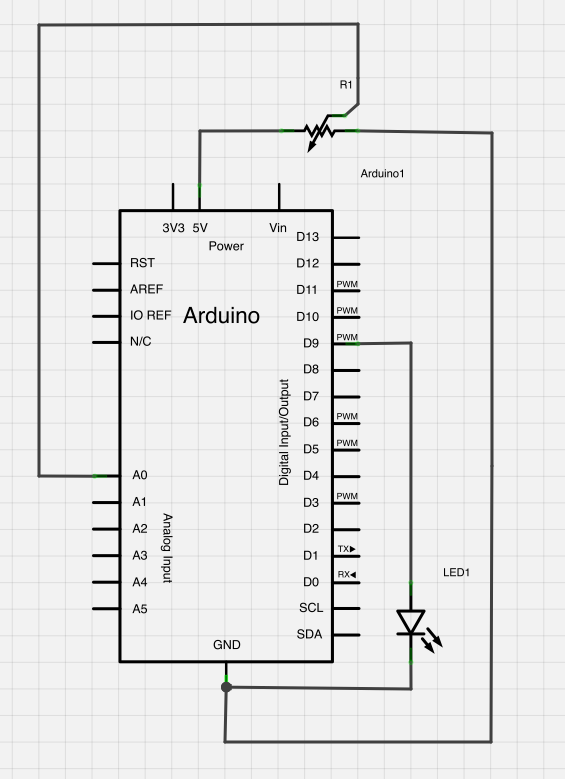
\includegraphics[height=4in]{figures/pot-fade.png}
    \caption{Arduino controlling brightness of an LED by reading an analog input value.}
    \label{fig:figures_pot-fade}
\end{figure}


Next, hook up a 10k potentiometer between the 5v and ground and middle leg to the A0 analog input on your Arduino as seen in Figure~\ref{fig:figures_pot-fade}.  Modify your \textbf{Fade} code to the code in Figure~\ref{fig:fade_mod}

\begin{figure}[htbp]
	\centering
\begin{minted}[mathescape,
				linenos,
				numbersep=5pt,
				gobble=0,
				frame=lines,
				framesep=2mm]{c}
const int led = 9;      // the pin that the LED is attached to
const int pot = A0;     // A0 will be the analog input channel
int sensorValue = 0;    // this will store the value read from the pot
int outputValue = 0;    // this is the value sent to our pwm pin

void setup()  { 
  pinMode(led, OUTPUT); // declare pin 9 to be an output
  Serial.begin(9600); // Open a serial monitor at 9600 baud
} 
void loop()  { 
  sensorValue = analogRead(pot); // store pot value in sensorValue
  outputValue = map(sensorValue, 0, 1023, 0, 255); // map sensorValue to correct range
  analogWrite(led, outputValue); // write the analog out value to led:
  
  Serial.print("sensor = " ); // print the results to the serial monitor:
  Serial.print(sensorValue);      
  Serial.print("\t output = ");      
  Serial.println(outputValue); 

  delay(2);  // wait 2 milliseconds for daq to settle 
}
\end{minted}
	\caption{The blink program modified to control the LED with a Potentiometer}
	\label{fig:fade_mod}
\end{figure}

\subsubsection{Understanding the changes to \textbf{Fade}} % (fold)
\label{ssub:understanding_the_changes_to_fade}

We declared a few new variables to keep track of an analog input pin and variables used for storing values from our analog input readings and our PWM output values.  See the comments in the code for more context.  

We also used the 
\texttt{Serial.begin(9600);} line in our \texttt{void setup()} loop to tell the Arduino that we want to open a serial communication session with our computer (remember how we picked a serial port in Section~\ref{sub:selecting_a_serial_port}?).

Outputting data to the serial line is a nice way to tell what is going on in your code, but remember that your program will run no faster than the speed of your serial line.

The next new piece of code is \texttt{analogRead(pot);}.  This does what it sounds like.  It reads the 0-5\emph{v} input on pin \texttt{pot} and converts it to a value between 0 and 1023.

We can only output PWM values analogous to 0 and 5\emph{v} by writing a value between 0 and 255 to our led pin.  Lucky we have a useful command called \texttt{map ()} which handles the analog input range to PWM output range conversion for us.  See the \texttt{map} info page for more details.\cite{map}

Next we write the adjusted input value to our \texttt{led} pin using \texttt{analogWrite(led, outputValue);}. 

Finally we print these input and output values the the serial line using the \texttt{Serial.print(value);} command.  \textbf{Open the serial monitor now to view these values in real time.  Go to \emph{Tools} $\rightarrow$  \emph{Serial Monitor}}.  You should see the input and output values similar to Figure~\ref{fig:figures_serial-mon}.

\begin{figure}[htbp]
    \centering
        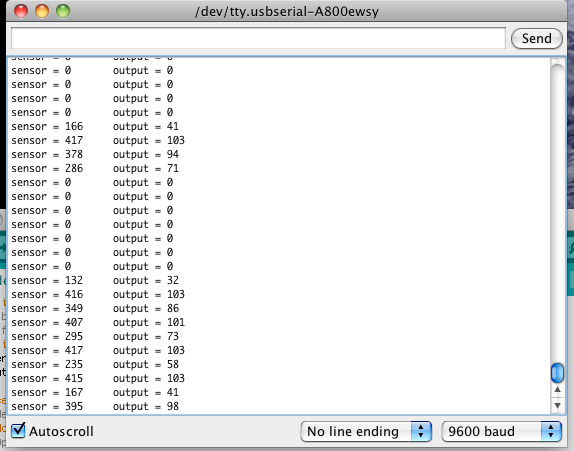
\includegraphics[height=1.8in]{figures/serial-mon.png}
    \caption{The serial monitor in action}x
    \label{fig:figures_serial-mon}
\end{figure}

% subsubsection understanding_the_changes_to_fade (end)
% subsubsection potentiometer (end)

\subsection{Photo Resistor} % (fold)
\label{sub:photo_resistor}

\textbf{Remove the potentiometer and wire in a photo-resistor as seen in Figure~\ref{fig:figures_photo-res}.}  A photo-resistor has a variable resistance depending on how much light is hitting it. 
\begin{figure}[htbp]
    \centering
        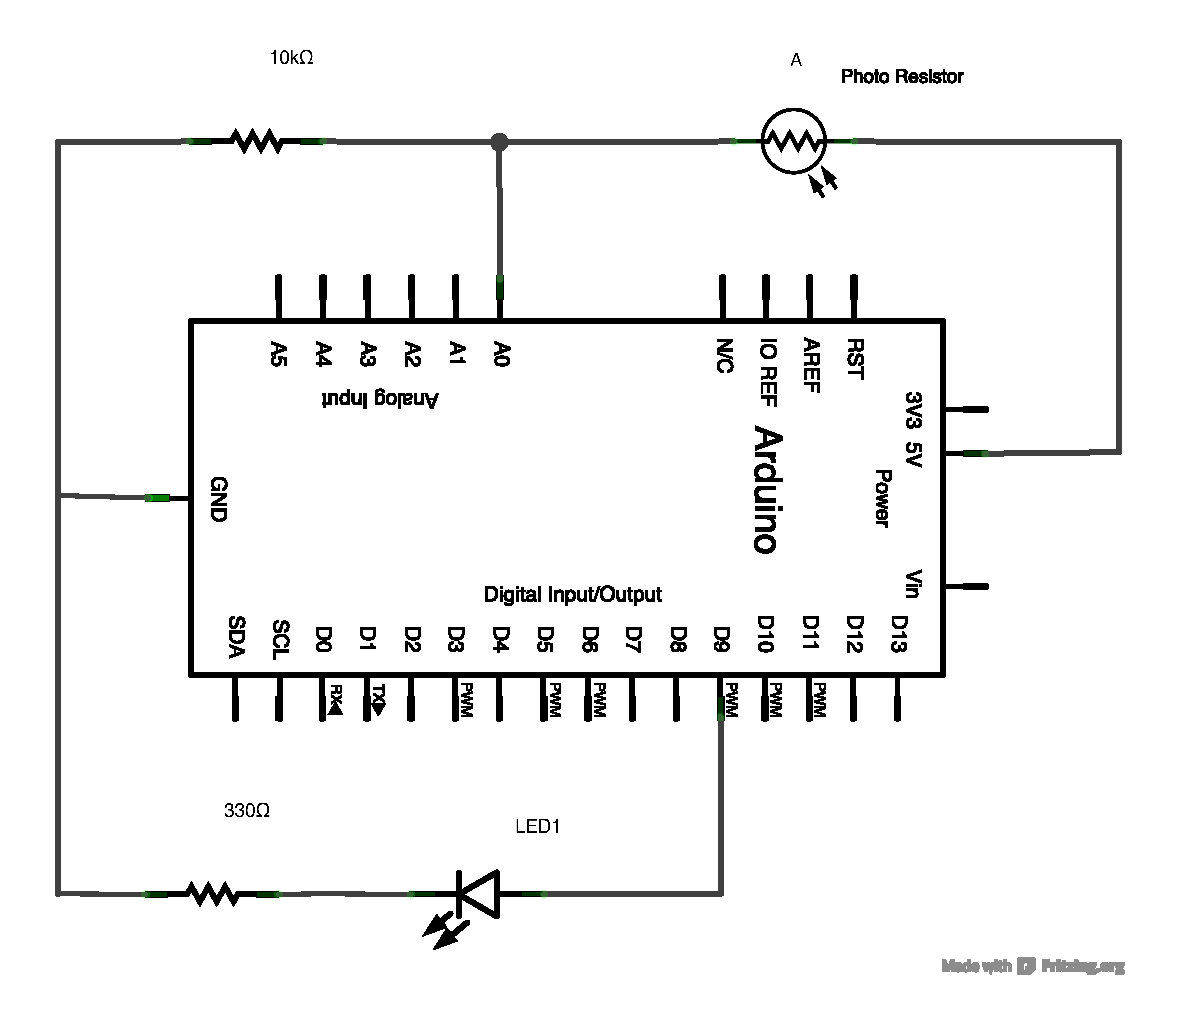
\includegraphics[height=3.5in]{figures/photo-res.png}
    \caption{Photo-resistor wired to A0}
    \label{fig:figures_photo-res}
\end{figure}

Using the same code as in Section~\ref{sub:potentiometer}, observe the output of the photo resistor and the PWM output on pin 9 simultaneously on your oscilloscope.  \textbf{Vary the amount of light hitting the photo-resistor and observe and compare the PWM output and voltage across the photo-resistor.}    

% subsection photo_resistor (end)

% subsection understanding_pwm (end)

% section using_inputs_to_control_outputs (end)

\section{PID and LEDs} % (fold)
\label{sec:pid_and_leds}

PID (Proportional, Integral, Differential) is way to control a system and take into account any kind error in your control mechanism.   There are there primary components to think about in a PID control loop. You have voltage corresponding to the current state of your system (position, temperature, etc) that is called your ``Process Variable'' or $PV$.  You also have a setpoint ($SP$) voltage, corresponding to the state you wish your $PV$ to reach.  Third, you have a control voltage, $u$, which corresponds to the instantaneous voltage value you are using to drive your system towards its $SP$ voltage.

The PID algorithm is show in Equation~\ref{eqn:pid}.


\begin{equation}
    \label{eqn:pid}
    u(t) = MV(t) = K_{p} e(t) + K_{i} \int _{0}^t e(\tau)d\tau + K_{d} \frac{d}{dt}e(t)
\end{equation}
% section pid_and_leds (end)

There is a proportional, integral and differential part to Equation~\ref{eqn:pid}.  The constants $K_{p}$, $K_{i}$, and $K_{d}$ are used to set the sign and contribution gain of each part of this equation.  $e(t)$ is your proportional ``error'' corresponding to $SP - PV$.  The variable $t$ corresponds to the current time in our system, and $\tau$ is simply a variable of integration.  

The proportional portion of the equation takes into account how far away our $PV$ is from our $SP$.  The differential part takes into account how fast we are moving (if we move to fast near our $SP$, we will over shoot), and can be used to reduce the proportional portion if we are moving to fast, or speed us up if we are experiencing resistance despite our proportional contribution.  

The integral part of the equation takes into account how long we have been off of the set point, contributing more to our output the longer we are missing the $SP$.  This is important because our P and D contributions will typically lead our $PV$ to sag slightly above or below our $SP$ variable.\cite{pid}

\subsection{Installing Libraries} % (fold)
\label{sub:installing_libraries}

\subsubsection{Windows} % (fold)
\label{ssub:windows_libraries}

% subsubsection windows (end)

\subsubsection{OS X} % (fold)
\label{ssub:os_x_libraries}

% subsubsection os_x (end)

% subsection installing_libraries (end)

\subsection{Using the PID Library} % (fold)
\label{sub:using_the_pid_library}

% subsection using_the_pid_library (end)

\section{PID Temperature Control} % (fold)
\label{sec:pid_temperature_control}

Controlling the temperature using PID and a fan.

% section pid_temperature_control (end)

\section{PID Extras} % (fold)
\label{sec:pid_extras}

\subsection{Implementing your own PID algorithm} % (fold)
\label{sub:implementing_your_own_pid_algorithm}

\subsection{Auto-tuning PID} % (fold)
\label{sub:auto-tuning_pid}

% subsection incorporating_ (end)

% subsection implementing_your_own_pid_algorithm (end)

% section pid_extras (end)

\section{Communicating With other Devices} % (fold)
\label{sec:communicating_with_other_devices}

Opening serial ports and talking to humans and computers.

% section communicating_with_other_devices (end)

\bibliography{references} 
\bibliographystyle{plain} \nocite{*}

\end{document}